%%%%%%%%%%%%%%%%%%%%%%%%%%%%%%%%%%%%%%%%%
% Class Notes Template
% LaTeX Template
% By: Ryan Grove
%%%%%%%%%%%%%%%%%%%%%%%%%%%%%%%%%%%%%%%%%

%----------------------------------------------------------------------------------------
%	PACKAGES AND OTHER DOCUMENT CONFIGURATIONS
%----------------------------------------------------------------------------------------

\documentclass[paper=a4, fontsize=11pt]{scrartcl} % A4 paper and 11pt font size

\usepackage[T1]{fontenc} % Use 8-bit encoding that has 256 glyphs
\usepackage{fourier} % Use the Adobe Utopia font for the document - comment this line to return to the LaTeX default
\usepackage[english]{babel} % English language/hyphenation
\usepackage{amsmath,amsfonts,amsthm} % Math packages

\usepackage{lipsum} % Used for inserting dummy 'Lorem ipsum' text into the template

\usepackage{sectsty} % Allows customizing section commands
\allsectionsfont{\centering \normalfont\scshape} % Make all sections centered, the default font and small caps

\usepackage{fancyhdr} % Custom headers and footers
\pagestyle{fancyplain} % Makes all pages in the document conform to the custom headers and footers
\fancyhead{} % No page header - if you want one, create it in the same way as the footers below
\fancyfoot[L]{} % Empty left footer
\fancyfoot[C]{} % Empty center footer
%\fancyfoot[R]{\thepage} % Page numbering for right footer
\renewcommand{\headrulewidth}{0pt} % Remove header underlines
\renewcommand{\footrulewidth}{0pt} % Remove footer underlines
\setlength{\headheight}{13.6pt} % Customize the height of the header

\numberwithin{equation}{section} % Number equations within sections (i.e. 1.1, 1.2, 2.1, 2.2 instead of 1, 2, 3, 4)
\numberwithin{figure}{section} % Number figures within sections (i.e. 1.1, 1.2, 2.1, 2.2 instead of 1, 2, 3, 4)
\numberwithin{table}{section} % Number tables within sections (i.e. 1.1, 1.2, 2.1, 2.2 instead of 1, 2, 3, 4)

\setlength\parindent{0pt} % Removes all indentation from paragraphs - comment this line for an assignment with lots of text

\usepackage{lastpage}
\usepackage{fancyhdr}
\cfoot{\thepage\ of \pageref{LastPage}}

\def\v{\hbox{$\mathbf v$}}
\def\w{\hbox{$\mathbf w$}}
\def\u{\hbox{$\mathbf u$}}
\def\x{\hbox{$\textbf{x}$}}
\def\z{\hbox{$\mathbf z$}}
\def\a{\hbox{$\mathbf a$}}
\def\b{\hbox{$\mathbf b$}}
\def\L{\hbox{$\mathcal L$}}
\def\C{\hbox{$\mathbb C$}}
\def\B{\hbox{$\mathcal B$}}
\def\R{\hbox{$\mathbb R$}}
\def\X{\hbox{$\underline X$}}
\def\Q{\hbox{$\mathbb Q$}}
\def\R{\hbox{$\mathbb R$}}
\def\N{\hbox{$\mathbb N$}}
\def\C{\hbox{$\mathbb C$}}
\def\0{\hbox{$\mathbf 0$}}
\def\Y{\hbox{$\underline Y$}}
\def\a{\hbox{$\mathbf a$}}
\def\u{\hbox{$\mathbf u$}}
\def\w{\hbox{$\mathbf w$}}
\def\y{\hbox{$\mathbf y$}}
\def\X{\hbox{$\underline X$}}
\def\dd{\hbox{$\partial $}}
\def\B{\hbox{$\mathcal B$}}
\def\F{\hbox{$\mathcal F$}}
\def\L{\hbox{$\mathcal L$}}
\def\M{\hbox{$\mathcal M$}}
\def\D{\hbox{$\mathscr {D}$}}
\def\RR{\hbox{$\mathscr{R}$}}
\def\I{\hbox{$\mathcal I$}}

\usepackage{amssymb}
%\theoremstyle{plain}
\usepackage[margin = .75in]{geometry}
\newtheorem{claim}{Claim}
\newtheorem{theorem}{Theorem}[section]
\newtheorem{lemma}[theorem]{Lemma}
\newtheorem{proposition}[theorem]{Proposition}
\newtheorem{corollary}[theorem]{Corollary}
\newtheorem{problem}[theorem]{Problem}
%\theoremstyle{definition}
\newtheorem{definition}[theorem]{Definition}
%\theoremstyle{remark}
\newtheorem{remark}[theorem]{Remark}
\newtheorem{remarks}[theorem]{Remarks}
\newtheorem{example}[theorem]{Example}
\newcommand{\ds}{\displaystyle}
\newcommand{\ZZ}{\mathbb{Z}}
\newcommand{\QQ}{\mathbb{Q}}
\newcommand{\e}{\varepsilon}
\newcommand{\bbf}{\textbf}
\newcommand{\p}{\parallel}
\usepackage{color}
\newcommand{\field}[1]{\mathbb{#1}}
\usepackage{amsmath}
\usepackage{amsthm}
\usepackage{amssymb}
\usepackage{mathrsfs}
\usepackage{cancel}
\usepackage{upgreek}
\usepackage{graphicx}
\usepackage{multirow}
\usepackage{setspace}
\usepackage{url}
\usepackage{subfigure}
\usepackage{enumerate}
\usepackage{cases}
\usepackage{mathrsfs}
\usepackage{rotating}

%----------------------------------------------------------------------------------------
%	TITLE SECTION
%----------------------------------------------------------------------------------------

\newcommand{\horrule}[1]{\rule{\linewidth}{#1}} % Create horizontal rule command with 1 argument of height

\title{	
\normalfont \normalsize 
\textsc{Ryan Grove, Clemson University, MATH1080 - 9} \\ [25pt] % Your name, university, class
\horrule{0.5pt} \\[0.4cm] % Thin top horizontal rule
\huge Section 11.1: Sequences \\ % The assignment title
\horrule{2pt} \\[0.5cm] % Thick bottom horizontal rule
}

\author{Date:} % The due date

\date{\normalsize February 23, 2016} % A custom date

\begin{document}

\maketitle % Print the title

\begin{flushleft}
\begin{tabular}{l l}
Name: \rule{3.2in}{.01cm}  & {}%Table number: \rule{1in}{.01cm}\\
\end{tabular}
\end{flushleft}

%----------------------------------------------------------------------------------------
%	Lecture
%----------------------------------------------------------------------------------------

\section*{\textbf{Lecture:}}
A \textbf{sequence} can be thought of as a list of numbers written in a definite order:
\[a_1,a_2,a_3,a_4,\ldots,a_n,\ldots\]

The number $a_1$ is called the \textit{first term}, $a_2$ is the \textit{second term}, and in general $a_n$ is the \textit{nth term}. We will deal exclusively with infinite sequences and so each term $a_n$ will have a successor $a_{n+1}$.\\
\indent

Notice that for every positive integer $n$ there is a corresponding number $a_n$ and so a sequence can be defined as a function whose domain is the set of positive integers. But we usually write $a_n$ instead of the function notation $f(n)$ for the value of the function at the number $n$.\\
\indent

\fbox{
  \parbox{\textwidth}{
  \vspace{5pt} \textbf{\underline{Notation}}: The sequence $\{a_1,a_2,\ldots,a_n,\ldots\}$ is also denoted by
  
  \[\{a_n\} \quad \text{ or } \quad \{a_n\}_{n=1}^\infty\]
  
  }}
  \indent\\
  \indent
  
  \underline{Example 1}: Some sequences can be defined by giving a formula for the $n$th term. In the following examples we give three descriptions of the sequence: one by using the preceding notation (above), another by using the defining formula, and a third by writing out the terms of the sequence. Notice that $n$ doesn't have to start at 1.
 \[ \begin{array}{rlll}
  (a) & \lbrace\ds\frac{n}{n+1}\rbrace_{n=1}^\infty \quad \quad & a_n = \ds\frac{n}{n+1} & \lbrace\ds\frac{1}{2},\ds\frac{2}{3},\ds\frac{3}{4},\ds\frac{4}{5},\ldots,\ds\frac{n}{n+1},\ldots\rbrace\\
  \text{ }\\
  (b) & \lbrace\ds\frac{(-1)^n(n+1)}{3^n}\rbrace & a_n = \ds\frac{(-1)^n(n+1)}{3^n} & \lbrace-\ds\frac{2}{3},\ds\frac{3}{9},-\ds\frac{4}{27},\ds\frac{5}{81},\ldots,\ds\frac{(-1)^n(n+1)}{3^n},\ldots\rbrace\\
  \text{ }\\
  (c) & \lbrace\ds\sqrt{n-3}\rbrace_{n=3}^\infty & a_n = \ds\sqrt{n-3}, \text{ } n\geq 3 \quad & \lbrace0,1,\sqrt{2},\sqrt{3},\ldots,\sqrt{n-3},\ldots\rbrace\\
  \text{ }\\
  (d) & \lbrace\cos\ds\frac{n\pi}{6}\rbrace_{n=0}^\infty \quad \quad & a_n = \cos\ds\frac{n\pi}{6},\text{ } n\geq 0 \quad \quad & \lbrace1,\ds\frac{\sqrt{3}}{2},\ds\frac{1}{2},0,\ldots,\cos\ds\frac{n\pi}{6},\ldots\rbrace\\
  \end{array}\]
  \indent
 \newpage

\underline{Example 2}: Find a formula for the general term $a_n$ of the sequence

\[\lbrace{\ds\frac{3}{5},-\ds\frac{4}{25},\ds\frac{5}{125},-\ds\frac{6}{625},\ds\frac{7}{3125},\ldots\rbrace}\]

assuming that the pattern of the first few terms continues.\\
\indent

\vspace{2in}

\underline{Example 3}: Here are some sequences that don't have a simple defining equation.\\
\begin{enumerate}
\item[(a)] The sequence $\{p_n\}$, where $p_n$ is the population of the world as of January 1 in the year $n$.\\
\item[(b)] If we let $a_n$ be the digit in the $n$th decimal place of the number $e$, then $\{a_n\}$ is a well-defined sequence whose first few terms are 
\[\{7,1,8,2,8,1,8,2,8,4,5,\ldots\}\]
\item[(c)] The \textbf{Fibonacci sequence} $\{f_n\}$ is defined recursively by the conditions
\[f_1=1 \quad f_2=1 \quad f_n=f_{n-1} + f_{n-2} \quad n\geq 3\]
Each term is the sum of the two preceding terms. The first few terms are
\[\{1,1,2,3,5,8,13,21,\ldots\}\]
This sequence arose when the 13th-century Italian mathematician known as Fibonacci solved a problem concerning the breeding of rabbits.\\
\end{enumerate}
\indent
\hrule
\indent

In general, the notation
\[\ds\lim_{n\to\infty}a_n = L\]
means that the terms of the sequence $\{a_n\}$ approach $L$ as $n$ becomes large. \\
\indent

\fbox{
  \parbox{\textwidth}{
  \vspace{5pt} \textbf{\underline{Definition 1}}: A sequence $\{a_n\}$ has the \textbf{limit} $L$ and we write
  
  \[\ds\lim_{n\to\infty}a_n=L \quad \text{ or } \quad a_n\to L \text{ as } n\to\infty\]
  
  if we can make the terms $a_n$ as close to $L$ as we like by taking $n$ sufficiently large.\\
  \begin{itemize}
  \item If $\ds\lim_{n\to\infty}a_n$ exists, we say the sequence \underline{\hspace{1.25in}} (or is \underline{\hspace{1.25in}}).\\
  \item Otherwise, we say the sequence \underline{\hspace{1.25in}} (or is \underline{\hspace{1.25in}}).\\
  \end{itemize}
  
  }}
  \indent\\
  \indent
  
  A more precise version of Definition 1 is as follows:\\
  \indent
  
  
  \fbox{
  \parbox{\textwidth}{
  \vspace{5pt} \textbf{\underline{Definition 2}}: A sequence $\{a_n\}$ has the \textbf{limit} $L$ and we write
  
 \[\ds\lim_{n\to\infty}a_n = L \quad \text{ or } \quad a_n\to L \text{ as } n\to \infty\]
 
 if for every $\epsilon> 0$ there is a corresponding integer $N$ such that
 \[\text{ if } \text{ } n>N \text{ } \text{ then } \text{ } |a_n-L|<\epsilon\]
 
 }}
 \indent\\
 \indent
 
 If you compare Definition 2 with Definition 2.6.7 (from MATH 1060) you will see that the only difference between $\ds\lim_{n\to\infty}a_n = L$ and $\ds\lim_{x\to\infty}f(x)=L$ is that $n$ is required to be an integer. Thus we have the following theorem:\\
 \indent
 
 \fbox{
  \parbox{\textwidth}{
  \vspace{5pt} \textbf{\underline{Theorem}}: If $\ds\lim_{x\to\infty}f(x)=L$ and $f(n)=a_n$ when $n$ is an integer, then $\ds\lim_{n\to\infty}a_n=L$.\\
  
  }}
  \indent\\
  \indent
  
  \fbox{
  \parbox{\textwidth}{
  \vspace{5pt} \textbf{\underline{Definition 3}}: $\ds\lim_{n\to\infty}a_n=\infty$ means that for every positive number $M$ there is an integer $N$ such that
  
  \[\text{ if } \text{ } n> N \text{ } \text{ then } \text{ } a_n>M\]
  
  }}
  \indent\\
  \indent
  
  If $\ds\lim_{n\to\infty}a_n=\infty$, then the sequence $\{a_n\}$ is divergent but in a special way. We say that $\{a_n\}$ diverges to $\infty$.\\
  \indent
  
  \textbf{\underline{Limit Laws}}:
  \[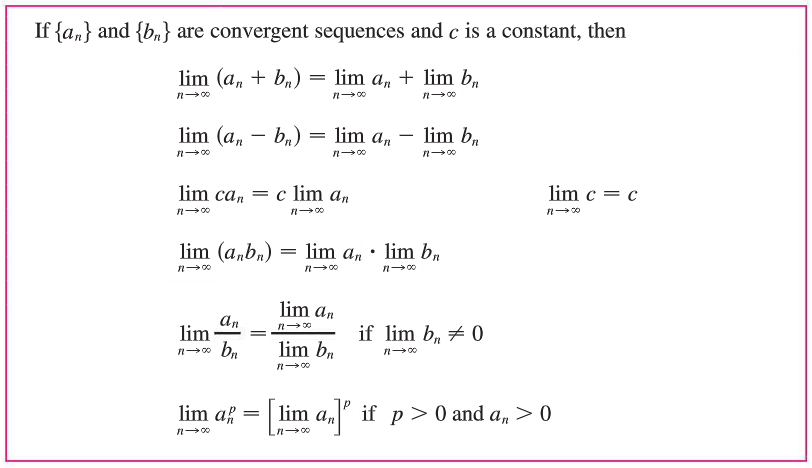
\includegraphics[scale=0.5]{11-1pic1.png}\]
  \indent
  
  \fbox{
  \parbox{\textwidth}{
  \vspace{5pt} \textbf{\underline{The Squeeze Theorem}}: 
  
  \[\text{If } a_n\leq b_n\leq c_n \text{ for } n\geq n_0 \text{ and } \ds\lim_{n\to\infty}a_n = \ds\lim_{n\to\infty}c_n = L, \text{ then } \ds\lim_{n\to\infty}b_n = L.\]
  
  }}
  \indent\\
  \indent
  
  Another useful fact:\\
  \indent
  
  \fbox{
  \parbox{\textwidth}{
  \vspace{5pt} \textbf{\underline{Theorem}}: \quad \quad If $\ds\lim_{n\to\infty}|a_n|=0, \text{ then } \ds\lim_{n\to\infty}a_n = 0$.\quad 
  }}
  \indent\\
  \indent
  
  \underline{Example 4}: Find $\ds\lim_{n\to\infty} \ds\frac{n}{n+1}$.\\
  \indent
  
  \textbf{Strategy}: Divide numerator and denominator by the highest power of $n$ that occurs in the denominator and then use the Limit Laws.
  
  \vspace{2.5in}
  
  \underline{Example 5}: Is the sequence $a_n = \ds\frac{n}{\ds\sqrt{10+n}}$ convergent or divergent?\\
  \indent
  
  \vspace{2.5in}
  
  \underline{Example 6}: Calculate $\ds\lim_{n\to\infty}\ds\frac{\ln n}{n}$.\\
  \indent
  
  \vspace{2.5in}
  \newpage
  \underline{Example 7}: Determine whether the sequence $a_n = (-1)^n$ is convergent or divergent.\\
  \indent
  
  \textbf{SOLUTION}: If we write out the terms of the sequence, we obtain: \text{ }$\{-1,1,-1,1,-1,1,-1,\ldots\}$.\\
  \indent
  
  The graph of the sequence is: 
  \vspace{-30pt}
  \[\quad \quad 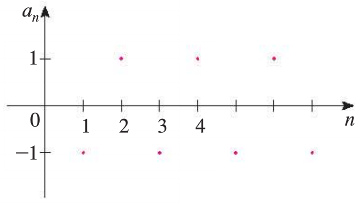
\includegraphics[scale=0.45]{11-1pic2.png}\]
  Since the terms oscillate between 1 and $-1$ infinitely often, $a_n$ does not approach any number. \\
  \indent
  
  Thus $\ds\lim_{n\to\infty}(-1)^n$ does not exist; that is, the sequence $\{(-1)^n\}$ is \underline{\hspace{1.25in}}.\\
\indent\\
\indent
  
  \underline{Example 8}: Evaluate $\ds\lim_{n\to\infty}\ds\frac{(-1)^n}{n}$ if it exists.\\
  \indent
  
  \textbf{SOLUTION}: We first calculate the limit of the absolute value:
  
  \vspace{2in}
  
  The following theorem says that if we apply a continuous function to the terms of a convergent sequence, the result is also convergent.\\
  \indent
  
  \fbox{
  \parbox{\textwidth}{
  \vspace{5pt} \textbf{\underline{Theorem}}: If $\ds\lim_{n\to\infty}a_n = L$ and the function $f$ is continuous at $L$, then
  \[\ds\lim_{n\to\infty}f(a_n) = f(L)\]
  }}
  \indent\\
  \indent
  
  \underline{Example 9}: Find $\ds\lim_{n\to\infty}\sin(\ds\frac{\pi}{n})$.\\
  \indent
  
  \vspace{1.6in}
  
  \underline{Example 10}: Discuss the convergence of the sequence $a_n=\ds\frac{n!}{n^n}$, where $n! = 1\cdot 2 \cdot 3 \cdot \cdots \cdot n$.\\
  \indent
  
  \textbf{SOLUTION}: Both numerator and denominator approach infinity as $n\to\infty$ but here we have no corresponding function for use with l'Hospital's Rule ($x!$ is not defined when $x$ is not an integer). Let's write out a few terms to get a feeling for what happens to $a_n$ as $n$ gets large:
  
  \[a_1=1 \quad \quad a_2 = \ds\frac{1\cdot 2}{2\cdot 2} \quad \quad a_3 = \ds\frac{1\cdot 2 \cdot 3}{3\cdot 3 \cdot 3} \quad \quad a_n = \ds\frac{1\cdot 2 \cdot 3 \cdot \cdots \cdot n}{n\cdot n \cdot \cdots \cdot n}\]
  
  We observe that we can write:
  \[a_n = \ds\frac{1}{n}\left(\ds\frac{2\cdot 3 \cdot \cdots \cdot n}{n\cdot n \cdot \cdots \cdot n}\right)\]
  
  Notice that the expression in parenthesis is at most 1 because the numerator is less than (or equal to) the denominator. So
  \indent
  
  \[\underline{\hspace{2in}}\]
  
  We know that $\ds\frac{1}{n}\to\underline{\hspace{0.3in}}$ as $n\to\infty$. Therefore,
  
  \[\underline{\hspace{4in}}\]
  \indent
  \indent
  
  \underline{Example 11}: For what values of $r$ is the sequence $\{r^n\}$ convergent?\\
  \indent
  
  \textbf{SOLUTION}: We know from the graphs of exponential functions that $\ds\lim_{x\to\infty}a^x = \infty$ for $a>1$ and $\ds\lim_{x\to\infty}a^x=0$ for $0<a<1$. Therefore,
  
  \[\ds\lim_{n\to\infty}r^n = \begin{cases}
  \infty & \text{ if } r>1\\
  0 & \text{ if } 0 < r < 1
  \end{cases}\]
  
  It is obvious that
  
  \[\ds\lim_{n\to\infty}r^n = \underline{\hspace{0.3in}} \quad \text{ and } \ds\lim_{n\to\infty}0^n = \underline{\hspace{0.3in}}\]
  
  If $-1<r<0$, then $0<|r|<1$, so
  
  \[\ds\lim_{n\to\infty}|r^n| = \ds\lim_{n\to\infty}|r|^n = 0 \quad \implies \quad \ds\lim_{n\to\infty}r^n = 0.\]
  
  If $r\leq -1$, then $\{r^n\}$ diverges as in Example 7. \\
  \indent
  
  
 \fbox{
  \parbox{\textwidth}{
  \vspace{5pt} The sequence $\{r^n\}$ is convergent if $-1 < r \leq 1$ and divergent for all other values of $r$.\\
  \[\ds\lim_{n\to\infty}r^n = \begin{cases}
  0 & \text{ if } -1<r<1\\
  1 & \text{ if } r=1
  \end{cases}\]
  
  }}
  \indent\\
  \indent
  
   \fbox{
  \parbox{\textwidth}{
  \vspace{5pt} \textbf{\underline{Definition 4}}: A sequence $\{a_n\}$ is called...
  \vspace{-5pt}
  \begin{itemize}
  \item \underline{\hspace{1.25in}} if $a_n < a_{n+1}$ for all $n\geq 1$.
  \item \underline{\hspace{1.25in}} if $a_n > a_{n+1}$ for all $n\geq 1$.
  \item \underline{\hspace{1.25in}} if it is either increasing or decreasing.
  \end{itemize}
  
  }}
  \indent\\
  \indent
  \newpage
  \underline{Example 12}: The sequence $\lbrace \ds\frac{3}{n+5}\rbrace$ is decreasing because...
  
  \vspace{1in}
  
  \indent
  
  \underline{Example 13}: Show that the sequence $a_n = \ds\frac{n}{n^2+1}$ is decreasing.\\
  \indent
  
  \textbf{SOLUTION 1}: We must show that $a_{n+1}<a_n$, that is,
  
  \[\ds\frac{n+1}{(n+1)^2+1}<\ds\frac{n}{n^2+1}\]
  
  \vspace{1.75in}
  
  Since $n\geq 1$, we know that the inequality $n^2+n>1$ is true. Therefore,
  
  \[\underline{\hspace{4in}}\]
  
 \indent
 
 \textbf{SOLUTION 2}: Consider the underlying function $f(x) = \ds\frac{x}{x^2+1}$.\\
 \indent
 
\vspace{2in}

\indent

 \fbox{
  \parbox{\textwidth}{
  \vspace{5pt} \textbf{\underline{Definition 5}}: A sequence $\{a_n\}$ is...
  \begin{itemize}
  \item \underline{\hspace{1.25in}} \underline{\hspace{1in}} if there is a number $M$ such that
  \[a_n\leq M \quad \text{ for all } n\geq 1\]
  \item \underline{\hspace{1.25in}} \underline{\hspace{1in}} if there is a number $m$ such that
  \[m\leq a_n \quad \text{ for all } n\geq 1\]
  \end{itemize}
  
  If it is bounded above or below, then $\{a_n\}$ is a \underline{\hspace{1.25in}} \textbf{sequence}.\\
  
  }}
  \indent\\
  \indent
  
  For instance, the sequence $a_n=n$ is bounded below ($a_n>0$) but not above. The sequence $a_n=\ds\frac{n}{n+1}$ is bounded because $0<a_n<1$ for all $n$.\\
  \indent
  
  We know that NOT every bounded sequence is convergent:
  \[a_n = (-1)^n \text{ satisfies } -1 \leq a_n \leq 1 \text{ but is divergent from Example 7}\]
  
  and NOT every monotonic sequence is convergent:
  \[a_n = n \text{ is increasing and thus monotonic, but } a_n = n \to\infty \text{ as } n\to\infty\]
  \indent
  
  BUT, if a sequence is BOTH \underline{\hspace{1.2in}} and \underline{\hspace{1.2in}}, then it must be \textbf{convergent}.\\
  \indent
  
  Intuitively, if $\{a_n\}$ is increasing and $a_n\leq M$ for all $n$, then the terms are forced to crowd together and approach some number $L$.
  
  \[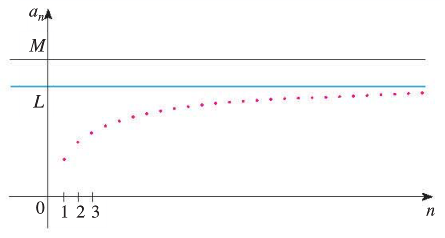
\includegraphics[scale=0.5]{11-1pic5.png}\]
  \indent
  
   \fbox{
  \parbox{\textwidth}{
  \vspace{5pt} \textbf{\underline{Monotonic Sequence Theorem}}: Every bounded, monotonic sequence is convergent.
  
  }}
  \indent\\
  \indent

















%----------------------------------------------------------------------------------------

\end{document}